% !TEX TS-program = pdflatexmk

\documentclass[a4paper, twoside]{article}

\usepackage{graphicx}
\usepackage[colorlinks]{hyperref}

\begin{document}

\title{Burden of Proof demo1b \\ Game Design Document}

\maketitle

\tableofcontents

\newpage

\section{Game}

\subsection{Overview}

\begin{itemize}
	\item{} genre : crime investigation video game ;
	\item{} demographics : 16+ ;
	\item{} TODO.
\end{itemize}

\newpage

\subsection{Gameplay}

TODO

\newpage

\subsection{City design}

City built from blueprint using parts specified in figure~\ref{fig:cityparts}.

\begin{figure}[h!tbp]
	\centering
	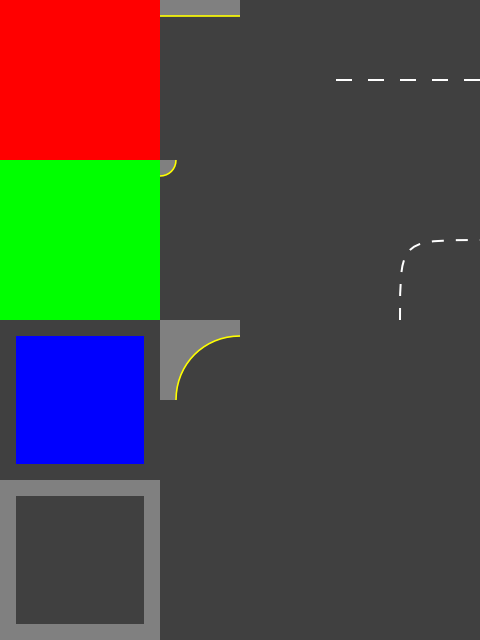
\includegraphics[width=0.8\textwidth]{images/cityparts.png}\ 
	\caption{City parts
		- First column : road block, ground block, building block, building pad
		- Second column : half sidewalk, interior sidewalk, exterior sidewalk
		- Third column : sraight markings, curved markings
		- Sidewalks have a roadside curb (yellow)}
	\label{fig:cityparts}
\end{figure}

\newpage

\section{Implementation}

\subsection{Code design}

\begin{figure}[h!tbp]
	\centering
	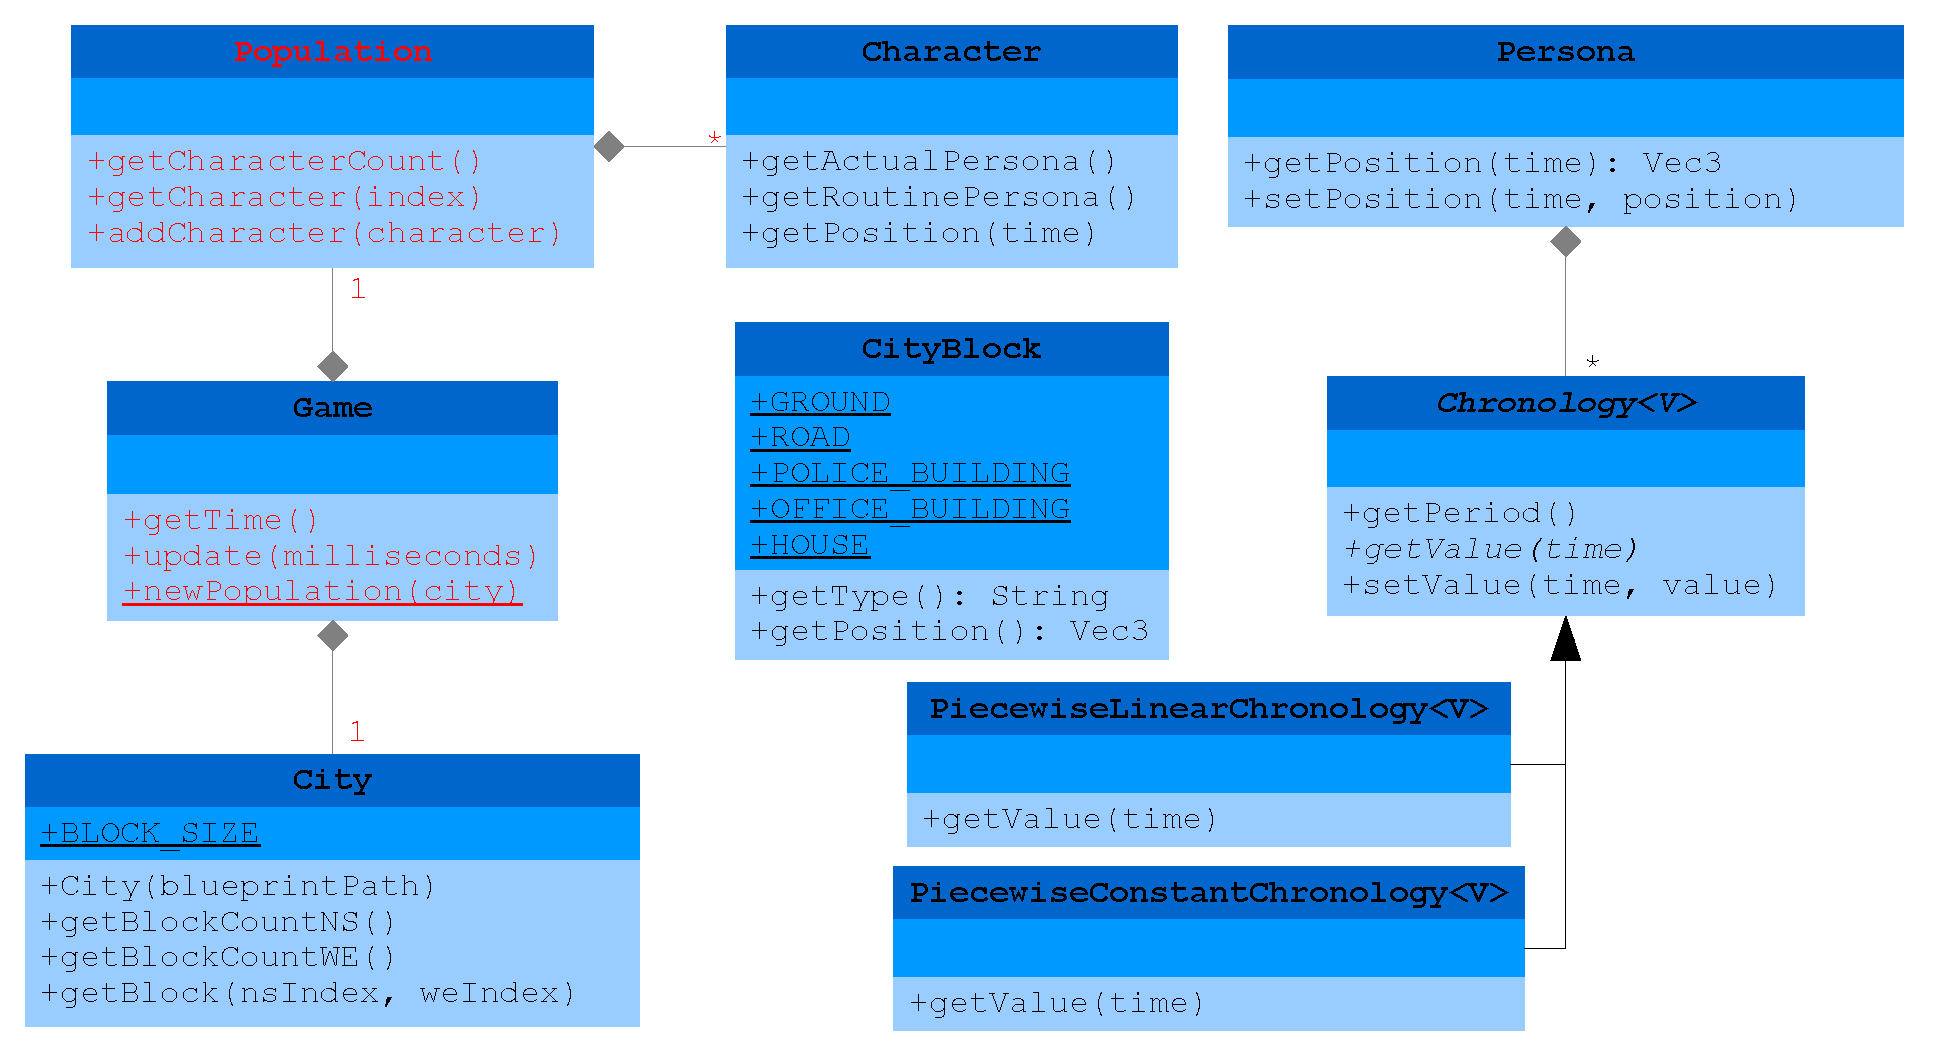
\includegraphics[width=1.0\textwidth]{images/classes.pdf}\ 
	\caption{Classes}
	\label{fig:classes}
\end{figure}

TODO: more UML diagrams

\newpage

\subsection{Coding conventions}

TODO

\end{document}
